\chapter{Theoretischer Hintergrund}
\section{Locks, Mutex}
Im Folgenden werden die Begriffe Lock und Mutex synonym verwendet.\\
Es gibt Situation in nebenläufigen Programmen, in denen sich verschiedene 
Routinen nicht gleichzeitig in bestimmten Bereichen aufhalten dürfen.\\
Locks gehören zu den am weitesten verbreiteten Mechanismen, um solche kritische 
Bereiche in einem Programm zu schützen \cite{zhou}.
Möchte ein Routine $R_1$ nun in einen Bereich 
eintreten, der durch ein Lock, welches bereits von einer anderen Routine $R_0$ 
gehalten wird, geschützt ist, muss sie so lange vor dem Lock warten, bis das Lock 
von $R_0$ wieder freigegeben wird.
\subsection{Operationen}
Auf Locks sind in der Regel die drei folgenden Operationen definiert.
\begin{itemize}
    \item Lock: Eine Routine $R$ versucht das Lock zu beanspruchen. Wird das Lock 
        von keiner Routine gehalten, wird das Lock geschlossen, so dass andere 
        Routinen es nicht beanspruchen können, bis es von $R$ wieder frei gegeben 
        wird. Ist es nicht möglich das Lock zu beanspruchen, da es bereits von 
        einer anderen Routine gehalten wird, muss $R$ so lange von der Operation 
        warten, bis eine Beanspruchung möglich ist.
    \item TryLock: TryLock unterscheidet sich von Lock dadurch, das die Routine,
        wenn es nicht möglich ist, das Lock zu beanspruchen nicht vor der 
        Operation wartet, sondern weiter ausgeführt wird, ohne das Lock beansprucht
        zu haben. Die Operation gibt außerdem zurück, ob die Beanspruchung 
        erfolgreich war.
    \item Unlock: Unlock gibt ein Lock wieder frei. Es kann nur von der Routine 
        frei gegeben werden, die es momentan hält.
\end{itemize}
\subsection{RW-Locks}
Neben den allgemeinen Locks gibt es noch s.g. Reader-Writer Locks. Diese haben im 
Vergleich zu den allgemeinen Locks zwei Lock und TryLock Operation, R-Lock und 
W-Lock (analog für TryLock). W-Lock, im folgenden einfach Lock genannt funktioniert 
identisch zu Lock in den allgemeinen Locks. Bei R-Locks hingegen ist es, anders 
als bei Lock, möglich, dass das Lock gleichzeitig von verschiedenen Routine gehalten wird
(oder mehrfach von der selben Routine), solange alle diese Beanspruchungen durch 
R-Lock erfolgt sind. Es ist nicht möglich ein Lock gleichzeitig durch R-Lock und 
Lock zu schließen.

\section{Deadlock} \label{Kap::Theo:Deadlocks}
\subsection{Zyklischer Deadlock}
Ein Deadlock ist ein Zustand in einem nebenläufigen Programm, also einem 
Programm, in dem mehrere Routinen nebenläufig ausgeführt werden, wobei alle 
laufenden Routinen zyklisch auf die Freigabe von Ressourcen warten.
Ein solcher Deadlock kann nun entstehen, wenn all Routinen vor einem Lock warten 
müssen, wobei die Locks immer von einer anderen Routine gehalten werden.\\
Man betrachte dazu das folgende Beispiel \cite{sulzmann} mit den Locks $x$ und $y$ 
und den beiden Routinen $R_1$ und $R_2$, welches den Ablauf eines Programms 
darstellt. $acq_i(l)$ bezeichnet dabei, dass das Lock $l$ von der Routine $R_i$ 
beansprucht und $rel_i(l)$, dass $l$ von $R_i$ wieder freigegeben wird.
\begin{table}[H]
    \centering
    \begin{tabular}{ccc}
       & $R_1$        & $R_2$          \\
    1. & $acq_{1}(y)$ &                \\
    2. & $acq_{1}(x)$ &                \\
    3. & $rel_{1}(x)$ &                \\
    4. & $rel_{1}(y)$ &                \\
    5. &              & $acq_{2}(x)$ \\
    6. &              & $acq_{2}(y)$ \\
    7. &              & $rel_{2}(y)$ \\
    8. &              & $rel_{2}(x)$
    \end{tabular}
\end{table}
Da $R_1$ und $R_2$ gleichzeitig ablaufen ist es möglich, dass sich die 
Reihenfolge der einzelnen Operationen zwischen den Routinen ändert (die Reihenfolge
innerhalb einer Routine ist immer gleich). Damit ist für das Programm, welches 
zu dem obigen Ablauf geführt hat, auch folgender Ablauf möglich. 
\begin{table}[H]
    \centering
    \begin{tabular}{ccc}
       & $R_1$          & $R_2$          \\
    1. & $acq_{1}(y)$ &                \\
    5. &                & $acq_{2}(x)$ \\
    2. & $B_2-acq_{1}(x)$ &                \\
    6. &                & $B_1-acq_{2}(y)$
    \end{tabular}
\end{table}
Dabei impliziert $B_j-acq_i(l)$, dass $acq_{i}(l)$ nicht ausgeführt werden konnte,
bzw. dass die Routine $R_i$ vor dem Lock halten muss, da das Lock bereits von 
Routine $R_j$ beansprucht wird. In diesem Beispiel wartet nun $R_1$ 
darauf, dass das Lock $x$ freigegeben wird und $R_2$ wartet darauf, dass Lock 
$y$ freigegeben wird. Da alle Routinen warten müssen, bis ein Lock freigegeben 
wird, allerdings keine der Routinen weiter laufen kann, um ein Lock freizugeben, 
kommt es zum Stillstand. Dieser Zustand wird als zyklischer Deadlock bezeichnet.
\subsection{Deadlock durch doppeltes Locking}\label{Kap::Theo:DoubleLocking}
Eine andere Situation, bei der ein Deadlock entstehen kann tritt auf, wenn 
eine Routine das selbe Lock mehrfach beansprucht, ohne es zwischendurch wieder 
freizugeben. Dies ist sogar möglich, wenn in dem Programm zu diesem Zeitpunkt
nur eine Routine aktiv ist. Ein Beispiel dafür gibt der folgende Programmablauf:
\begin{table}[H]
    \centering
    \begin{tabular}{cc}
        & $R_1$ \\
        1. & $acq_{1}(x)$ \\
        2. & $B_1-acq_1(x)$
    \end{tabular}
\end{table}
Die Routine muss dabei vor der zweiten Beanspruchung warten,
ohne dass es die Möglichkeit gibt, dass die Routine irgendwann weiter laufen wird.
Solch ein Deadlock wird als doppeltes Locking bezeichnet.\\
\section{Deadlocks-Detection}
Deadlocks in Programmen sind Fehler, die oft den vollständige Abbruch eines 
Programmes zu Folge haben, wenn keine zusätzliche Logik zur Erkennung und Auflösung von 
Deadlocks implementiert ist. Aus diesem Grund möchte man bereits bei der 
Implementierung eines Programms verhindern, dass ein solcher Deadlock auftreten 
kann. Unglücklicherweise kann es ohne zusätzliche Hilfsmittel schwierig sein, 
einen solchen Deadlock zu erkennen, da das Auftreten eines Deadlock von dem 
genauen zeitlichen Ablauf der verschiedenen Routinen abhängt.\\
Um dennoch Deadlocks 
erkennen zu können, können Lock-Graphen oder Lock-Bäume verwendet werden.
\subsection{Lock-Graphen}
Ein Lock-Graph ist ein gerichteter Graph $G = (L, E)$. Dabei ist $L$ die Menge 
aller Locks. $E \subseteq L \times L$ ist definiert als $(l_1, l_2) \in E$ genau 
dann, wenn es eine Routine $R$ gibt, auf welche $acq(l_2)$ ausgeführt wird, während sie 
bereits das Lock $l_1$ hält \cite{bensalem}. Mathematisch ausgedrückt gilt also 
\begin{align*}
    (l_1, l_2) \in E \Leftrightarrow \exists t_1, t_3\ \nexists t_2\ \exists i\ ((t_1 < t_2 < t_3) \land acq_i(l_1)[t_1] \land rel_i(l_1)[t_2] \land  acq_i(l_2)[t_3])
\end{align*}
wobei $acq_i(l_j)[t_k]$ bedeutet, dass $acq(l_i)$ zum Zeitpunkt $t_k$ auf Routine 
$j$ ausgeführt wird und equivalent für $rel_i(l_j)[t_k]$.\\
Ein Deadlock kann nun auftreten, wenn es innerhalb dieses Graphen einen Kreis 
gibt. Um zu verhindern, dass ein False-Positive dadurch ausgelöst wird, dass 
alle Kanten in einem solchen Kreis aus der selben Routine kommen (wodurch kein 
Deadlock entstehen kann), können die Kanten noch zusätzlich mit einem Label 
versehen werden, welches die Routine identifiziert, durch welche die Kante in 
den Graphen eingefügt wurde. Bei dem Testen nach Zyklen muss nun beachtet 
werden, dass nicht alle Kanten in dem Kreis das selbe Label haben 
\cite{bensalem}. Es sei zusätzlich noch gesagt, dass ein Zyklus in einem 
Lockgraphen nicht immer auf ein potenzielles Deadlock hinweist. Ein solcher 
Fall, bei dem die Detektion von Zyklen zu einer fälschlichen Detektion 
führt, sind sogenannt Gate-Locks. Diese treten z.B. in folgender Situation
auf:
\begin{table}[H]
     \centering
     \begin{tabular}{ccc}
        & $R_1$        & $R_2$          \\
     1. & $acq_{1}(z)$ &                \\
     2. & $acq_{1}(y)$ &                \\
     3. & $acq_{1}(x)$ &                \\
     4. & $rel_{1}(x)$ &                \\
     5. & $rel_{1}(y)$ &                \\
     6. & $rel_{1}(z)$ &                \\
     7. &              & $acq_{2}(z)$ \\
     8. &              & $acq_{2}(x)$ \\
     9. &              & $acq_{2}(y)$ \\
    10. &              & $rel_{2}(y)$ \\
    11. &              & $rel_{2}(x)$ \\
    12. &              & $rel_{2}(z)$
    \end{tabular}
\end{table}
In diesem Fall bilden die Locks $x$ und $y$ in dem Lock-Graphen einen Zyklus. 
Allerdings verhindert das Lock $z$, dass in diesem Fall ein tatsächliches 
Deadlock auftreten kann, da sich immer nur eine der beiden Routinen 
in dem Bereich mit den Locks $x$ und $y$ aufhalten kann.

\subsection{Lock-Bäume} \label{Kap::Theo:LockTree}
Anders als bei Lock-Graphen, speichert bei Lock-Bäumen jede Routine  
seine eigenen Abhängigkeiten. Dies bedeutet, dass der Lock-Baum $B_i$ der 
Routine $R_i$ genau dann die Kante $x\to y$ besitzt, wenn in Routine $R_i$ das 
Lock $y$ beansprucht wird und $x$ das letzte Lock ist, welches von $R_i$ beansprucht 
worde ist, ohne das $x$ wider freigegeben wurde. 
Mathematisch ausgedrückt ist ein Lock-Baum $B_i = (L_i, E_i)$ für Routine $i$ also ein 
Baum, wobei $L_i$ eine Teilmenge der in der Routine vorkommenden Locks is, und 
die Menge der Kanten $E_i$ über
\begin{align*}
    (l_1, l_2) \in E_i \Leftrightarrow &\exists t_1, t_4\ \nexists t_2, t_3, l_3\\
    &((t_1 < t_2 < t_3 \lor t_1 < t_3 < t_2 < t_4) \land (\lnot l_1 = l_3 \land \lnot l_2 = l_3)\\
    & \land acq_i(l_1)[t_1] \land rel_i(l_1)[t_2] \land acq_i(l_3)[t_3] acq_i(l_2)[t_4])
\end{align*}
gegeben ist.\\
Im folgenden, wird ein Lock-Baum als eine Menge von Dependencies betrachtet. 
Eine solche Dependency besteht aus einem Lock \texttt{mu} und einer Menge von Locks \texttt{hs}
(\texttt{holdingSet}),
von denen \texttt{mu} anhängt, für die es also einen Pfad von $x$ nach $mu$ mit $x \in hs$ gibt.\\
Ein potenzielles Deadlock liegt nun vor, wenn es in der Menge aller Dependencies
eine gültige, zyklische Kette gibt.\\
Ein Pfad mit $n$
Elementen ist eine gültige Kette, wenn die folgenden Eigenschaften gelten:
\begin{align}
  &\forall\ i, j \in \{1,...,n\}\ (dep_i = dep_j) \rightarrow (i = j) \tag{\ref{Kap::Theo:LockTree}.a}
  \label{For::Theo:LockTree.a}\\
  &\forall\ i \in \{1,...,n\}\ mu_i \in hs_{i+1} 
  \tag{\ref{Kap::Theo:LockTree}.b}
  \label{For::Theo:LockTree.b}\\
  &\forall\ i \in \{1,...,n\}\ read(mu_i) \rightarrow 
  (\forall\ mu \in hs_{i+1}\ (mu = mu_i) \to \lnot read(mu))
  \tag{\ref{Kap::Theo:LockTree}.c}
  \label{For::Theo:LockTree.c}\\
  &\makecell{\forall\ i, j \in \{1,...,n\}\ \lnot (i = j) \rightarrow 
  (\exists\ mu_1 \in hs_i\ \exists\ mu_2 \in hs_j ((mu_1 = mu_2) \rightarrow\\
  (read(mu_1) \land read(mu_2))))\phantom{123123123122131231231231223123}}
  \tag{\ref{Kap::Theo:LockTree}.d}
  \label{For::Theo:LockTree.d}
\end{align}
Dabei bezeichnet $mu_i$ den Mutex und $hs_i$ das holdingSet der $i$-ten 
Dependency $dep_i$ in der Kette. $read(mu)$ ist wahr, wenn das Locking von $mu$, welches 
in der Dependency abgebildet ist durch ein R-Lock zustande gekommen ist.\\
\eqref{For::Theo:LockTree.a} stellt sicher, dass die selbe 
Dependency nicht mehr als ein mal in der Kette auftauchen kann.  
\eqref{For::Theo:LockTree.b} besagt, dass die Dependencies tatsächlich
eine Kette bilden müssen, dass also der Mutex einer Dependency immer in dem 
HoldingSet der nächsten Dependency in dem Pfad enthalten sein muss. 
Auch wenn dies wahr ist, ist dies dennoch keine gültige Kette, wenn sowohl der
Mutex $mu_i$ als auch der Mutex $mu$ in $hs_{i+1}$, für die $mu = mu_i$ gilt, 
beides Reader-Locks sind. Dass solche Pfade ausgeschlossen werden wird durch 
\eqref{For::Theo:LockTree.c} sichergestellt. Die letzte Formel 
\eqref{For::Theo:LockTree.d} beschäftigt sich mit Gate-Locks. 
Sie besagt, dass wenn es einen Mutex gibt, 
der in den HoldingSets zweier verschiedener Dependencies in dem Pfad vorkommt, 
so müssen beide diese Mutexe Reader-Locks sein. Sind sie es nicht, handelt es 
sich um Gate-Locks, und der entsprechende Pfad kann somit nicht zu einem 
Deadlock führen. Wenn diese vier Formeln erfüllt sind, handelt es sich um eine 
gültige Kette.\\
Ein potenzielles Deadlock ergibt sich nun, wenn diese Kette einen Zyklus 
bildet, wenn als 
\begin{align}
  &mu_n \in hs_{1} 
  \tag{\ref{Kap::Theo:LockTree}.e}
  \label{For::Implementation:Periodical.e}\\
  &read(mu_n) \rightarrow 
  (\forall\ mu \in hs_{1}: (mu = mu_n) \to \lnot read(mu))
  \tag{\ref{Kap::Theo:LockTree}.f}
  \label{For::Implementation:Periodical.f}
\end{align}
gilt.\\\\
Man betrachte das folgende Beispiel:
\begin{table}[H]
    \centering
    \begin{tabular}{cccc}
        & $R_1$           & $R_2$           & $R_3$\\
        1. & $acq_{1}(mu_1)$ & $acq_{2}(mu_2)$ & $acq_{3}(mu_3)$ \\
        2. & $acq_{1}(mu_2)$ & $acq_{2}(mu_3)$ & $acq_{3}(mu_1)$ \\
        3. & $rel_{1}(mu_2)$ & $rel_{2}(mu_3)$ & $rel_{3}(mu_1)$\\
        4. & $rel_{1}(mu_1)$ & $rel_{2}(mu_2)$ & $rel_{3}(mu_3)$\\
        5. & $acq_{1}(mu_4)$ &                 & \\
        6. & $acq_{1}(mu_5)$ &                 & \\
        7. & $acq_{1}(mu_6)$ &                 & \\
        8. & $rel_{1}(mu_6)$ &                 & \\
        9. & $rel_{1}(mu_5)$ &                 & \\
        10. & $rel_{1}(mu_4)$ &                 & \\
   \end{tabular}
\end{table}
Hierbei wird nur die Programme der einzelnen Routinen dargestellt, 
nicht aber der Ablauf zwischen den Routinen.\\
Dabei gibt sich die Menge der Dependencies für $R1$ zu 
\begin{align*}
    B_1 = \{(mu_2, \{mu_1\}), (mu_5, \{m_4\})(mu_6, \{mu_5, mu_4\})\}
\end{align*}
für $R_2$ zu 
\begin{align*}
    B_2 = \{(mu_3, \{mu_2\}\})\},
\end{align*}
und für $R_3$ zu 
\begin{align*}
    B_3 = \{(mu_1, \{mu_3\}\})\},
\end{align*} wobei eine Dependency immer als Tuple der Form $(mu, hs)$ angegeben 
wird. Dies lässt sich folgendermaßen graphisch darstellen:
\begin{figure}[H]
    \centering
    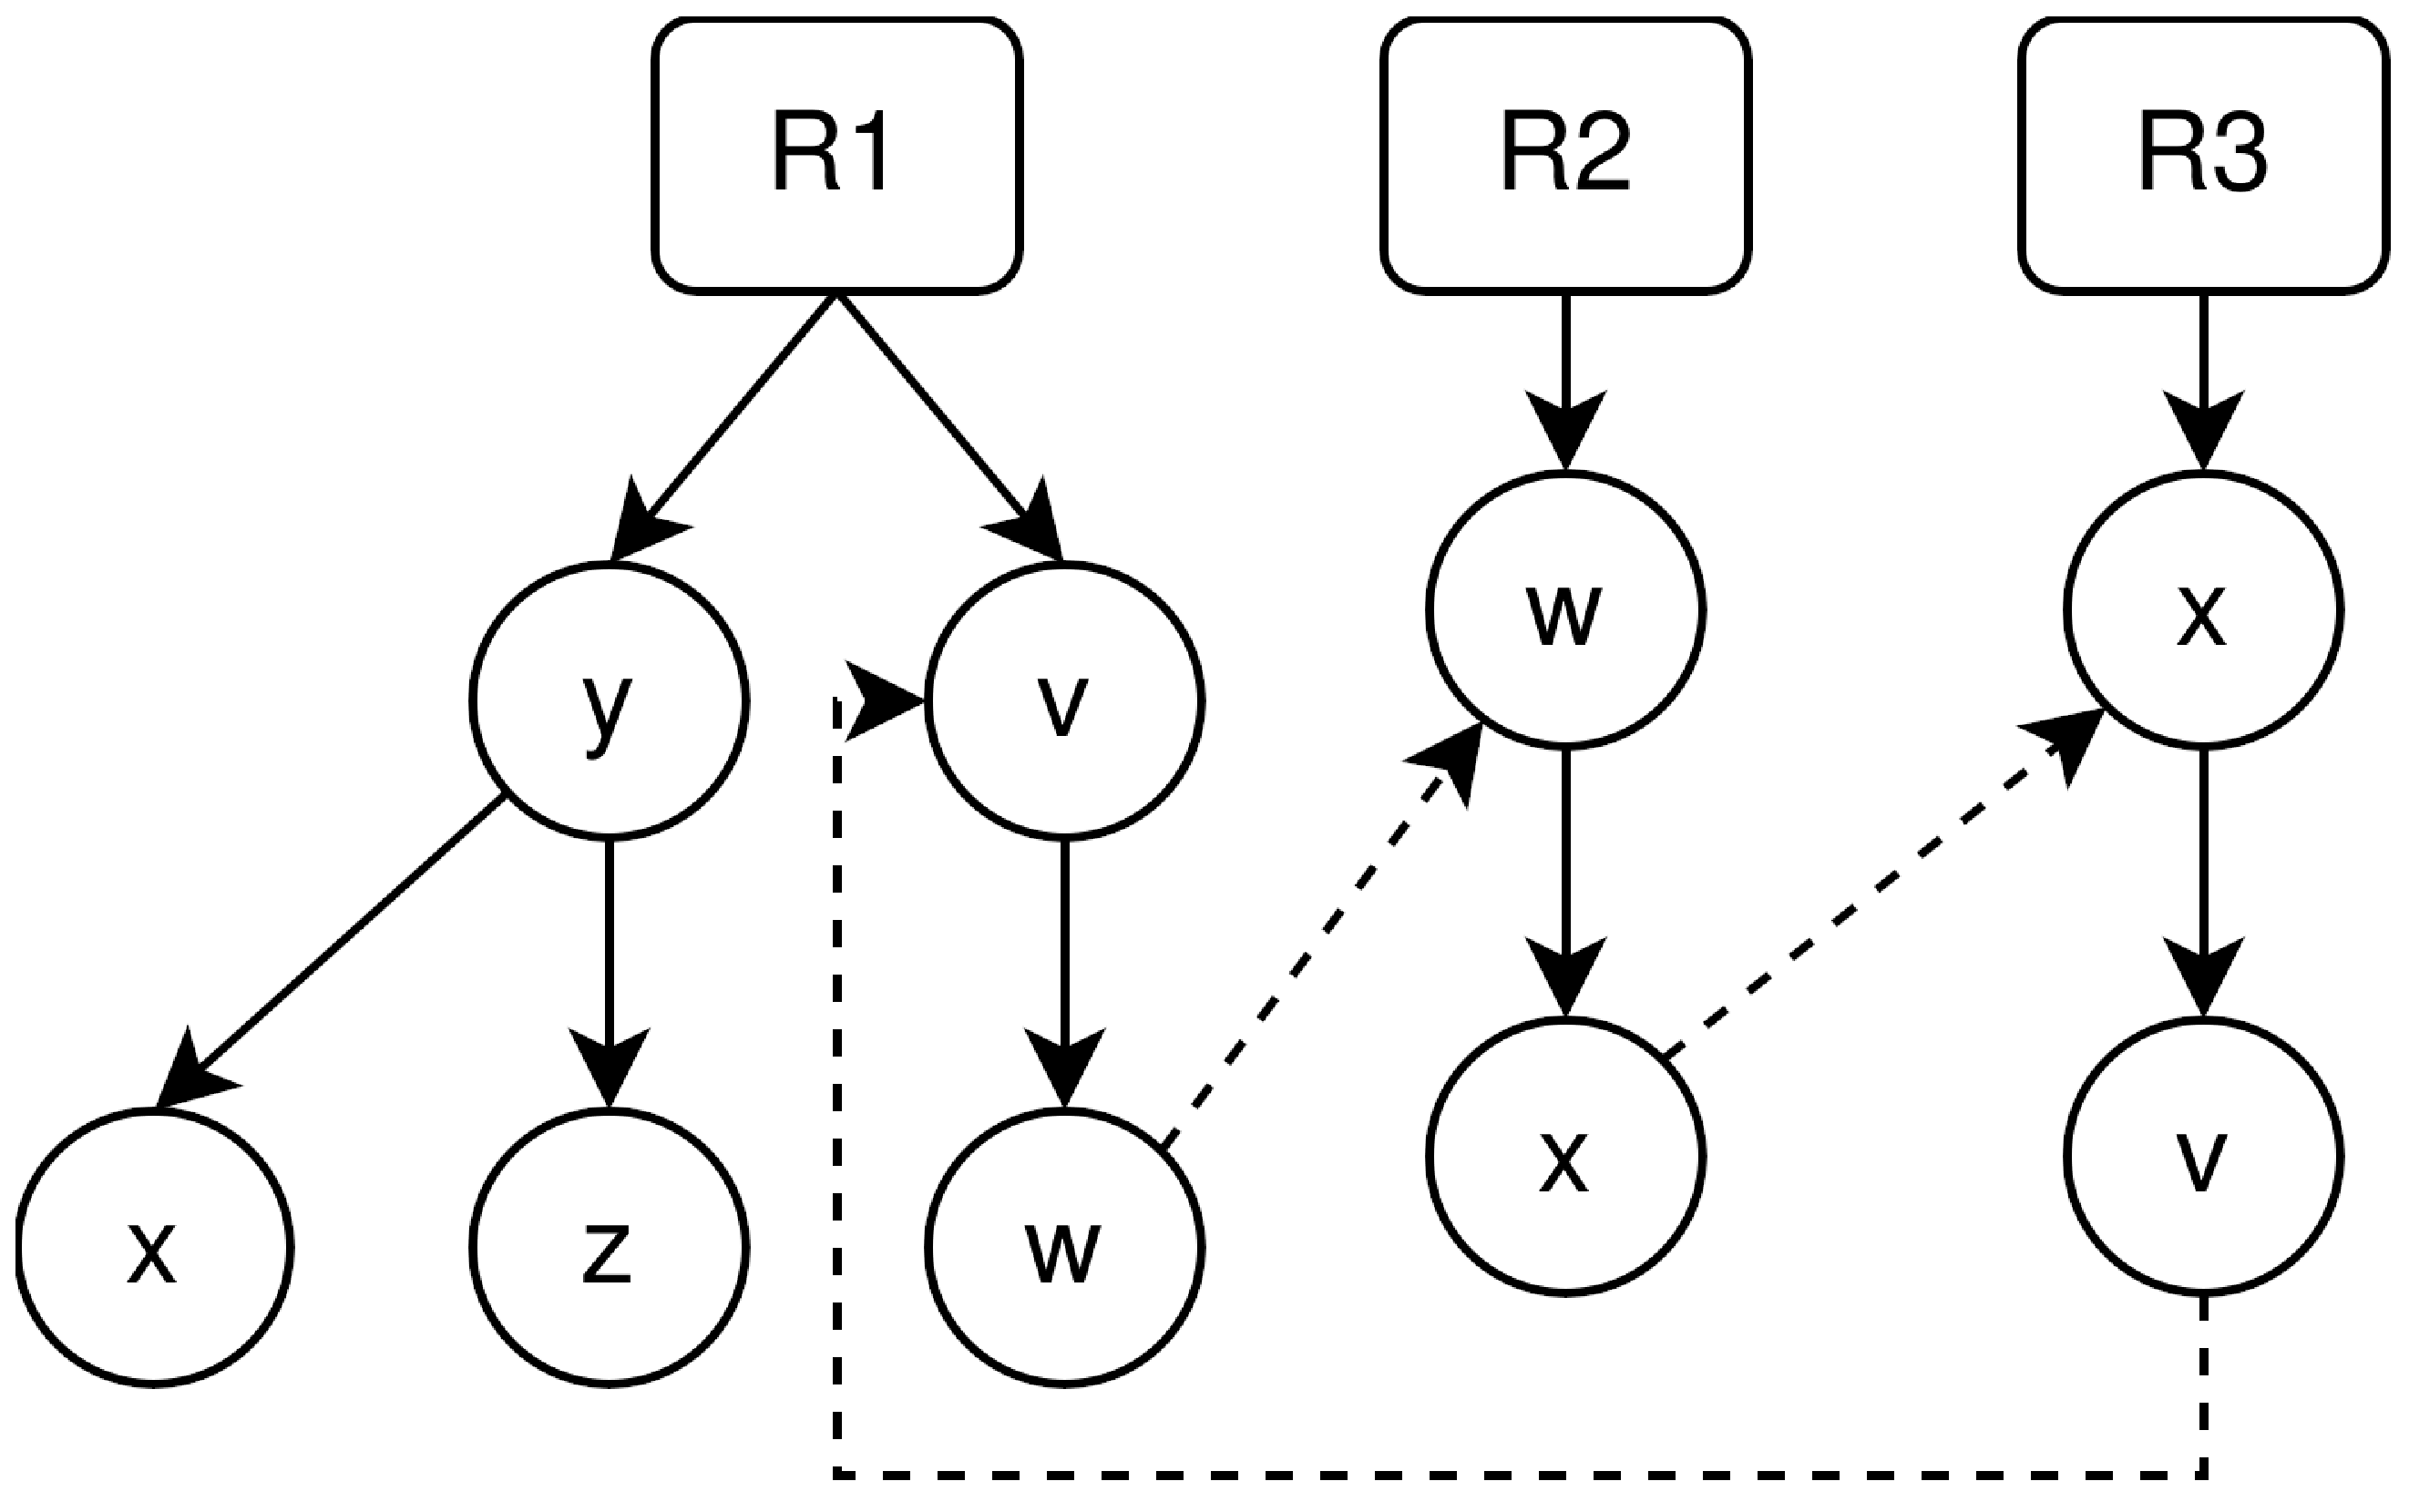
\includegraphics[width=.47\textwidth]{img/tree_example.eps}
    \caption{Graphische Darstellung der Lock-Bäume aus dem Beispiel. Die Knoten 
    entsprechen dabei Locks. Die durchgezogenen Pfeile repräsentieren die Kanten 
    der Lock-Bäume. Die gestichelten Kanten zeigen den enthaltenen Zyklus an.}
\end{figure}
Verbindet man nun 
gleiche Locks zwischen den einzelnen Bäumen (im Bild mit gestrichelten Pfeilen),
besitzt der entstehende Graph einen Zyklus zwischen $mu_1, mu_2$ und $mu_3$. 
Solch ein Zyklus indiziert einen potentiellen Deadlock.\\\\
Diese Verwendung von Lock-Bäumen hat mehrere Vorteile gegenüber Lock-Graphen. 
Da jede Routine ihre 
eigene Datenstruktur hat, wird verhindert, dass es durch 
gleichzeitigen Zugriff verschiedener Routinen auf die selbe Datenstruktur zu 
Problemen kommt. Zudem muss die Zugehörigkeit der Abhängigkeiten zu 
verschiedenen Routinen nicht explizit gespeichert werden. Ein weiterer Vorteil 
besteht darin, dass bei der Erkennung von Deadlocks mit Lock-Bäumen Situationen,
die aufgrund von Gate-Locks nicht zu Deadlocks führen können, automatisch nicht
als Deadlock erkannt werden, während es bei Lock-Graphen in solchen Fällen ohne 
zusätzliche Tests zu falschen Meldungen kommt.  

\subsection{Doppeltes Locking}
Doppeltes Locking, wie in Kapitel \ref{Kap::Theo:DoubleLocking} beschrieben,
 lässt sich nicht aus den Lock-Graphen oder Lock-Bäumen erkennen.\\
Es ist daher notwendig diese gesondert zu betrachten. Dazu speichert jedes Lock, 
von welchen Routinen es momentan gehalten wird, und für welche dieser 
Beanspruchungen es über R-Lock beansprucht worden ist.\\
Währen dem (R-)(Try-)Lock Vorgang, noch bevor es zu der eigentlichen Beanspruchung 
kommt, wird überprüft, ob das Lock in der selben Routine bereits gehalten 
wird, ohne dass es sich bei beiden Operationen um R-Locks handelt. In diesem 
Fall kommt es zu einem Deadlock.
\section{UNDEAD} \label{Kap::Theo:UNDEAD}
UNDEAD \cite{zhou} ist ein Algorithmus zur Detektion tatsächlicher und 
potenzieller Deadlocks. Zusätzlich versucht er potenzielle Deadlocks 
in weiteren Durchläufen zu verhindern. Da sich dieses Projekt aber nur mit der 
Detektion von Deadlocks befasst, soll darauf nicht weiter eingegangen werden.\\\\ 
UNDEAD implementiert Drop-in-Replacements für Locks mit Lock, TryLock und Unlock
Operationen, mit denen nach potenziellen oder tatsächlichen Deadlocks gesucht 
werden soll. Der Algorithmus benutzt dabei eine Implementierung von Lock-Bäumen 
bestehend aus Dependencies.\\
Die Detektion in UNDEAD läuft in drei Phasen ab. Diese sind die Logging-Phase, 
die periodische Detektion und die abschließende Detektion.
\subsection{Logging-Phase}
Die Logging-Phase läuft während dem Ablauf des eigentlichen Programms und sammelt
Informationen, die zur Erkennung von potenziellen Deadlocks notwendig sind. 
Zusätzlich sammelt es Call-Stacks für Lock-Operationen. Wird eine Lock-Operation
oder eine erfolgreiche Try-Lock Operation ausgeführt, wird eine nue Dependency 
erstellt. Diese werden für jede Routine in einer separaten 
Hashtabelle gespeichert, um gleichzeitigen Zugriff mehrerer Routinen auf solche 
Strukturen zu verhin
dern. Als Schlüssel für die Tabelle wird dabei der XOr 
Wert der Speicheradressen zweier Locks verwendet. Wenn z.B. das Lock $l_1$ 
von den Locks $\{l_2, l_3\}$ abhängt, wird der XOr Wert der Speicheradressen der 
beiden innersten Locks (hier z.B. $l_1$ und $l_2$) als Schlüssel verhindert, um 
Konflikte zwischen den verschiedenen Schlüsseln zu verhindern. Diese 
Hashtabellen bilden damit die Implementierung der Lock-Bäume.\\\\
UNDEAD versucht die Menge der gesammelten Daten so weit wie möglich zu reduzieren.
Dies bedeutet, dass keine Call-Stacks für single-Level Locks (Locks, die von 
keinen anderen Locks abhängen) gespeichert werde.
Außerdem werden, wenn in dem Programm momentan nur eine Routine läuft keine 
Informationen gespeichert. Außerdem versucht UNDEAD, mehrfach auftretende
Dependencies nicht mehrfach zu speichern, und in diesem Fall auch die Call-Stack
Informationen nicht mehrfach abzufragen.
\subsection{Periodische Detektion}
Die periodische Detektion wird verwendet, um tatsächlich auftretende Deadlocks bereits während dem 
Ablauf des Programms zu erkennen. Dazu wird in regelmäßigen, zeitlichen 
Abständen eine Routine für die Detektion gestartet.\\
Jede Routine speichert eine 
aktuelle Dependency, also diejenige Dependency, die zuletzt erkannt wurde.
Wenn die periodische Routine gestartet wird, macht der Detektor einen Snapshot
dieser aktuellen Dependencies und sucht in diesen nach Zyklen, wie in Kap.
\ref{Kap::Theo:LockTree} beschrieben. Wird ein solcher Zyklus gefunden, wird 
überprüft, ob sich die Menge der aktuellen Dependencies seit dem Start der 
periodischen Detektion geändert hat. Ist dies der Fall, so geht UNDEAD davon aus,
dass es sich nur um ein potenzielles Deadlock handelt, welches aber nicht 
aufgetreten ist. In diesem Fall wird das Programm normal weiter ausgeführt.
Andernfalls geht UNDEAD davon aus, das ein tatsächliches Deadlock aufgetreten 
ist. Tritt dieser Fall auf, wird die 
abschließende Detektion (Kap. \ref{Kap::UNDEAD:Abschließende}) gestartet 
und das Programm im Anschluss abgebrochen. 
\subsection{Abschließende Detektion} \label{Kap::UNDEAD:Abschließende}
Die abschließende Detektion wird ausgeführt, nachdem das eigentliche Programm
abgeschlossen wurde, oder wenn sie durch die periodische Detektion gestartet wurde.
Die Detektion basiert dabei auf dem iGoodLock Methode 
zur Detektion von Deadlocks, basierend aud DeadlockFuzzer \cite{Joshi} und 
MagicFuzzer \cite{Cai}. Für die Detektion sucht UNDEAD nach Zyklen wie in Kap.
\ref{Kap::Theo:LockTree} (\eqref{For::Theo:LockTree.a} - \eqref{For::Theo:LockTree.d})
beschrieben. Dazu sucht es nach Dependency-Ketten 
durch Betrachtung aller möglichen Permutationen von Dependencies in zwei Routinen, dann 
in drei, usw. Es nutzt dabei 
eine Tiefensuche, um diese Ketten iterativ zu durchsuchen. Wenn eine solche Kette 
gefunden wurde, wird überprüft, ob sie einen Zyklus bildet 
(\eqref{For::Implementation:Periodical.e} - \eqref{For::Implementation:Periodical.f}).
Ein solcher Zyklus deutet auf einen potenziellen Deadlock hin, was dazu 
führt, dass UNDEAD eine Information über den gefundenen potenziellen Deadlock ausgibt.


